\chapter{Architektura aplikacji}
W rozdziale przedstawiono wymagania funkcjonalne i niefunkcjonalne, które zostały postawione aplikacji. Zaprezentowano również diagramy przypadków użycia, stanów oraz sekwencji.
\section{wymagania funkcjonalne}
Wymagania funkcjonalne określają zachowanie systemu i jego reakcji na określone zadania \cite{Wymagania}.
\begin{table}[!h]
	\centering
	\renewcommand{\arraystretch}{1.3}
	\setlength{\tabcolsep}{6pt}
	\begin{tabular}{|c|p{5cm}|p{8cm}|}
		\hline
		\textbf{Nr} & \textbf{Wymaganie funkcjonalne} & \textbf{Opis} \\ \hline
		
		1. & Rejestracja użytkownika & System umożliwia utworzenie konta użytkownika z danymi logowania. \\ \hline
		2. & Logowanie do systemu & System weryfikuje dane użytkownika i umożliwia dostęp do panelu aplikacji. \\ \hline
		3. & Sprawdzenie dostępnych środków & Użytkownik może sprawdzić ile posiada balansu na koncie. \\ \hline
		4. & Wpłata pieniędzy na konto & Użytkownik może zasilić konto. \\ \hline
		5. & Przegląd historii wydatków & Aplikacja wyświetla listę wszystkich wydatków. \\ \hline
		6. & Tworzenie przelewu & System pozwala stworzyć przelew użytkownikowi. \\ \hline
		7. & Podsumowanie finansów konta & Użytkownik może sprawdzić dane o swoich wydatkach dla danego konta. \\ \hline
		8. & Kategoryzowanie transakcji & Użytkownik może podać kategorię dla wpłat i wypłat z konta. \\ \hline
		9. & Prezentacja wydatków na wykresie & System wyświetla wykres z wydatkami za dzień, tydzień, miesiąc oraz rok. \\ \hline
	\end{tabular}
	\caption{Wymagania funkcjonalne systemu do zarządzania budżetem domowym}
	\label{tab:wymagania_funkcjonalne}
\end{table}

\section{Wymagania niefunkcjonalne}
Wymaganiami funkcjonalnymi nazywamy wszystkie potrzeby, które nie dotyczą funkcjonalności produktu \cite{Wymagania}. Wymagania te opisują m.in. jak szybko system powinien odpowiadać na żądania, w jakim czasie produkt ma zostać dostarczony, jak ma prezentować się interfejs użytkownika. 
\begin{table}[H]
	\centering
	\renewcommand{\arraystretch}{1.3}
	\setlength{\tabcolsep}{6pt}
	\begin{tabular}{|c|p{3.1cm}|p{9.9cm}|}
		\hline
		\textbf{Nr} & \textbf{Wymaganie niefunkcjonalne} & \textbf{Opis} \\ \hline
		
		1. & Niezawodność & System w krótkim czasie odzyskuje pełną funkcjonalność w przypadku wystąpienia błędu. \\ \hline
		2. & Dostępność & System ma być dostępna przez 99.5\% czasu działania serwera.\\ \hline
		3. & Wydajność & System reaguje na żądanie w czasie krótszym niż 1 sekunda. Może obsłużyć do 1000 użytkowników jednocześnie. System jest w stanie przetworzyć do 10 GB na godzinę.  System jest skalowalny.\\ \hline
		4. & Bezpieczeństwo & System zapewnia, że dane są dostępne tylko dla osób upoważnionych. Autoryzacja użytkowników odbywa się poprzez podanie odpowiedniego loginu oraz hasła. Hasła muszą być przechowywane w formie zaszyfrowanej. \\ \hline
		5. & Wdrożenie & Aplikacja serwerowa musi być uruchomiona w środowisku JVM oraz korzystać z wersji Java 21 , Warstwa prezentacji uruchamiana w środowisku NodeJs z wykorzystaniem 9 wersji biblioteki React. Dane przechowywane w postaci dokumentów bazy danych MongoDB w wersji 8, Aplikacja uruchomiana jest w środowisku systemu operacyjnego Windows 11 oraz Linux \\ \hline
		
	\end{tabular}
	\caption{Wymagania niefunkcjonalne systemu do zarządzania budżetem domowym}
	\label{tab:wymagania_niefunkcjonalne}
\end{table}
\section{Diagramy przypadków użycia}
Diagram przypadków użycia (ang. \textit{Use Case Diagram})
\begin{figure}[H]
	\centering
	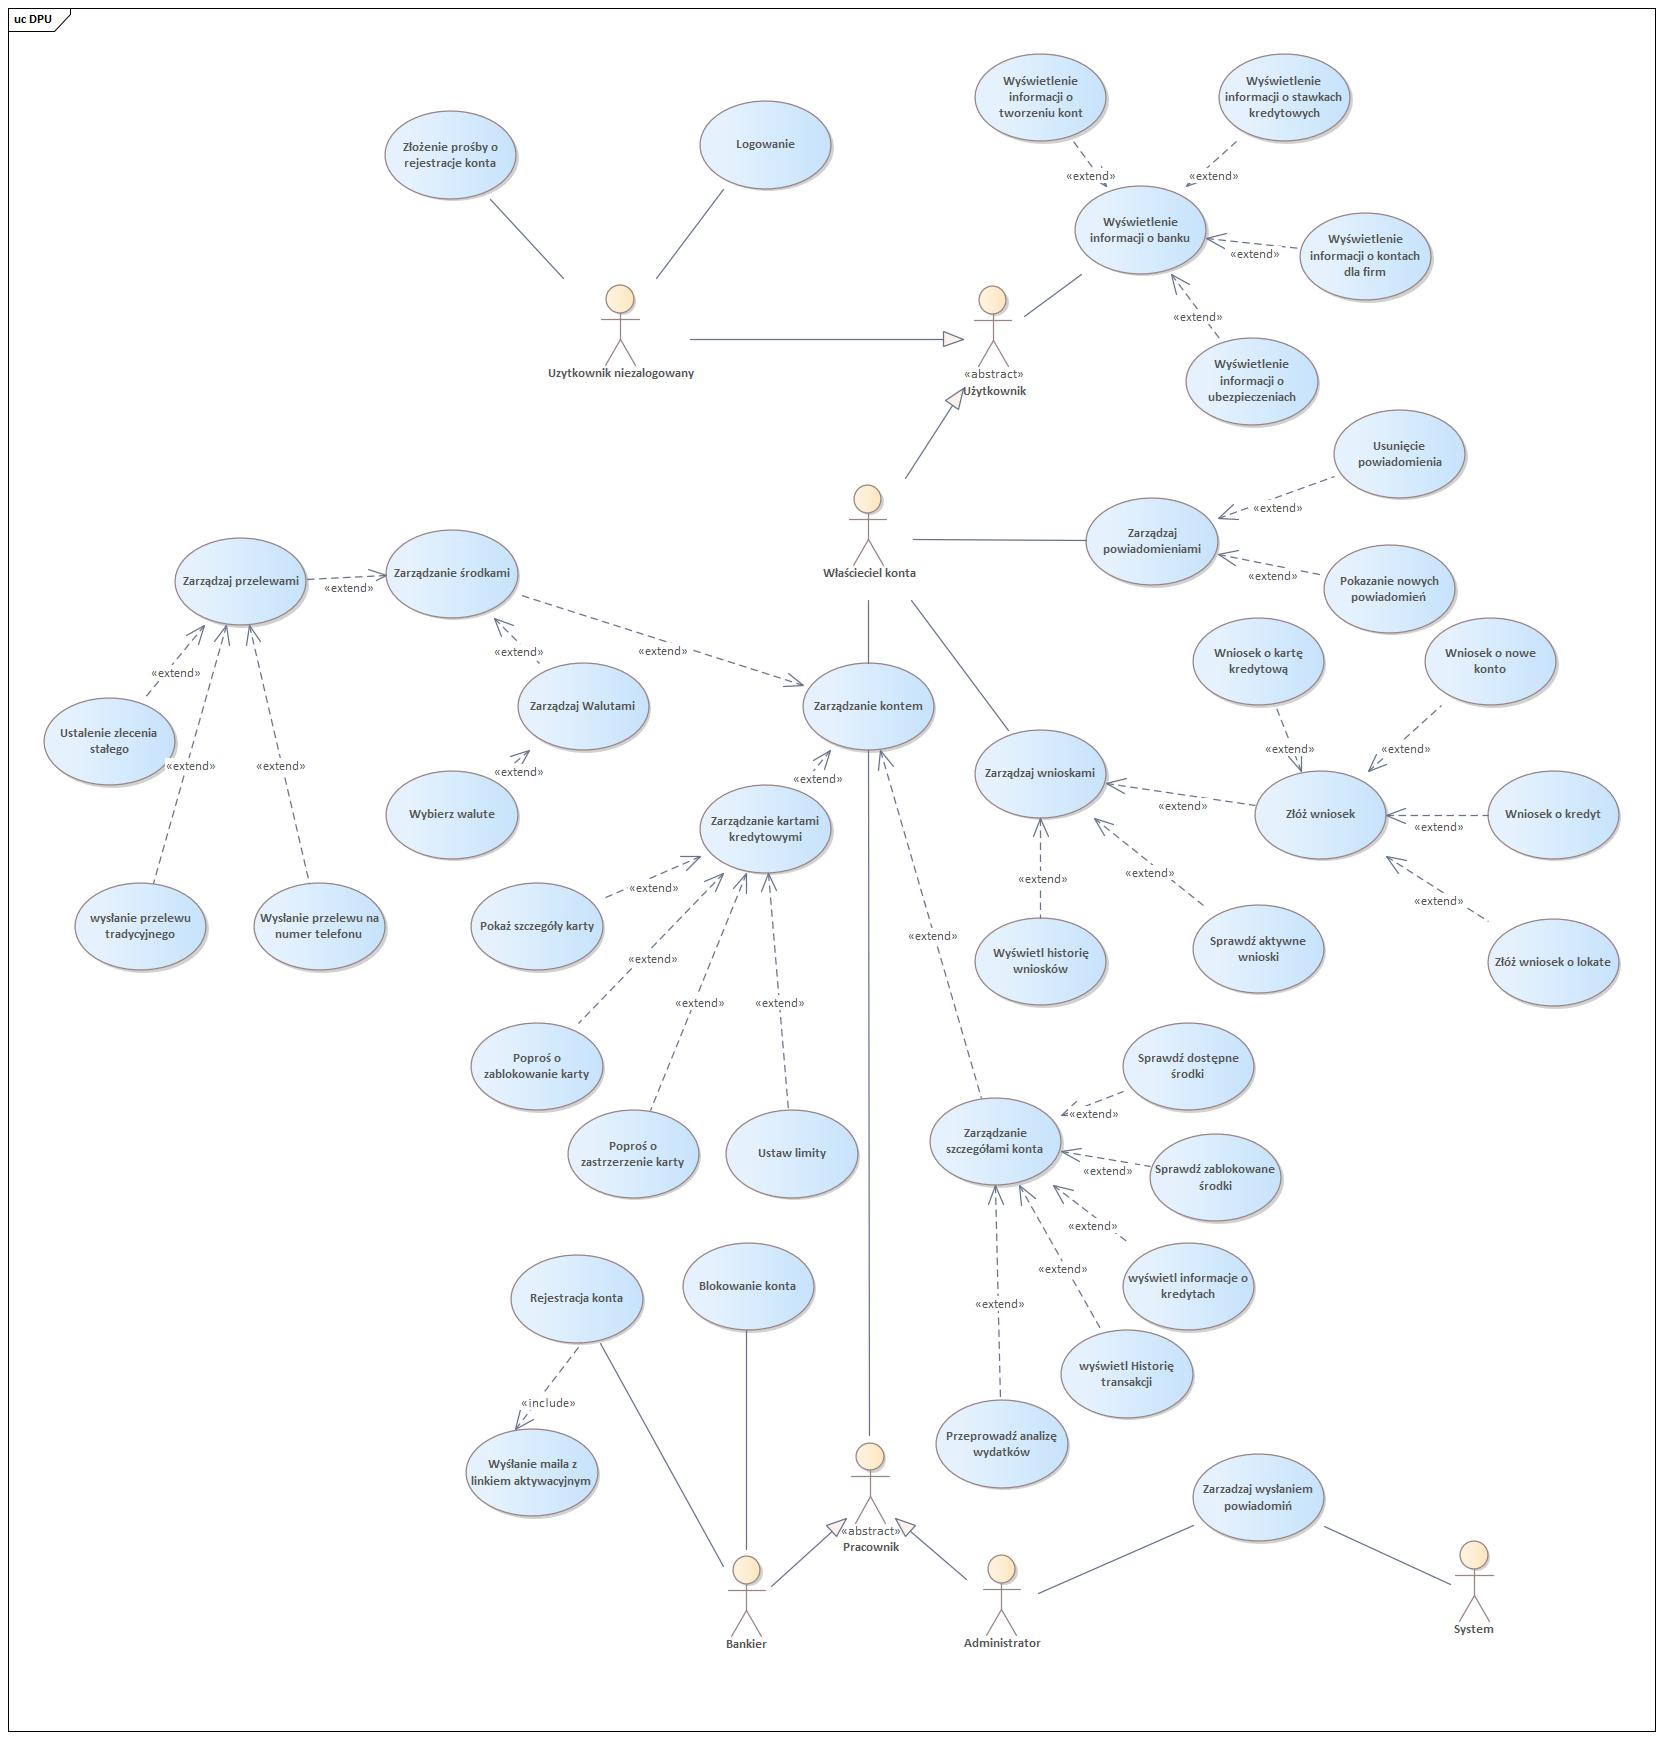
\includegraphics[width=1\textwidth]{images/DPU.jpg}
	\caption{Diagram przypadków użycia}
	\label{fig:UseCase}
\end{figure}
\section{Diagram stanów}
\begin{figure}[H]
	\centering
	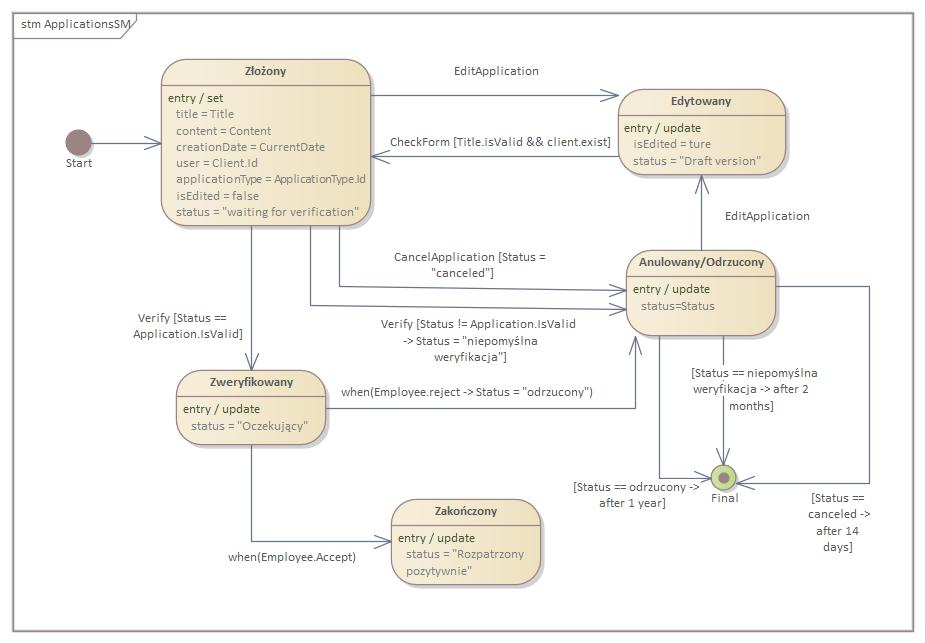
\includegraphics[width=1\textwidth]{images/Wniosek.jpg}
	\caption{Diagram stanów składania wniosku}
	\label{fig:StateMachine}
\end{figure}
\section{Diagramy sekwencji}
\begin{figure}[H]
	\centering
	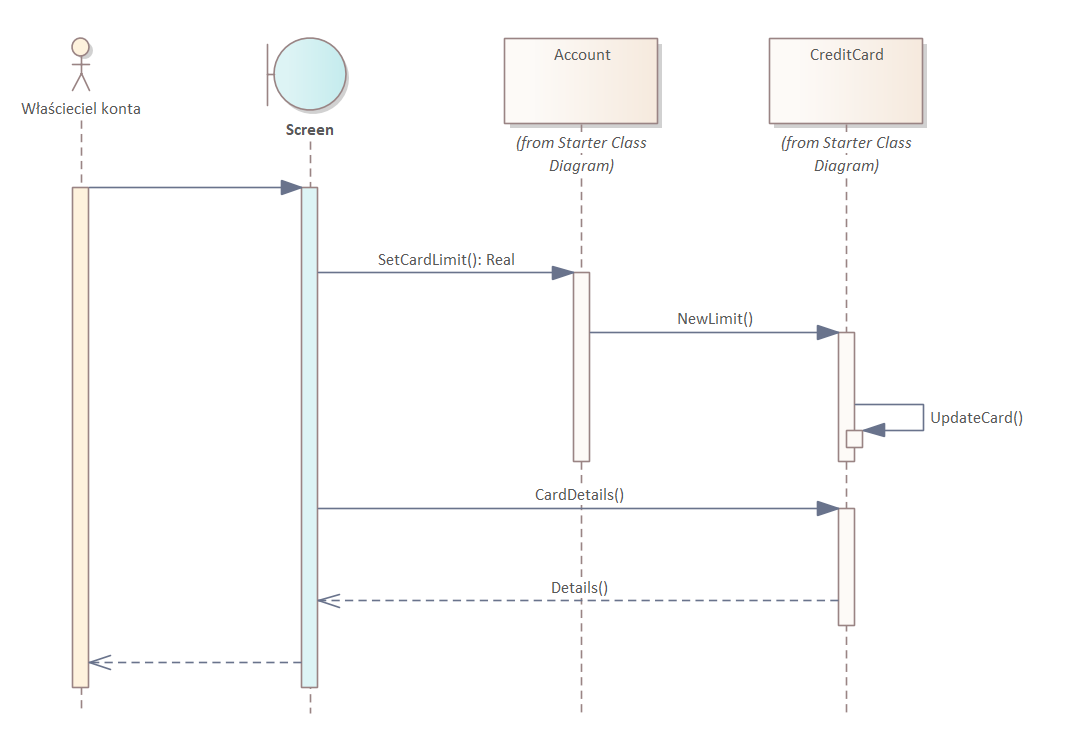
\includegraphics[width=0.7\textwidth]{images/Limit.png}
	\caption{Diagram sekwencji Limit}
	\label{fig:Seq1}
\end{figure}
\begin{figure}[H]
	\centering
	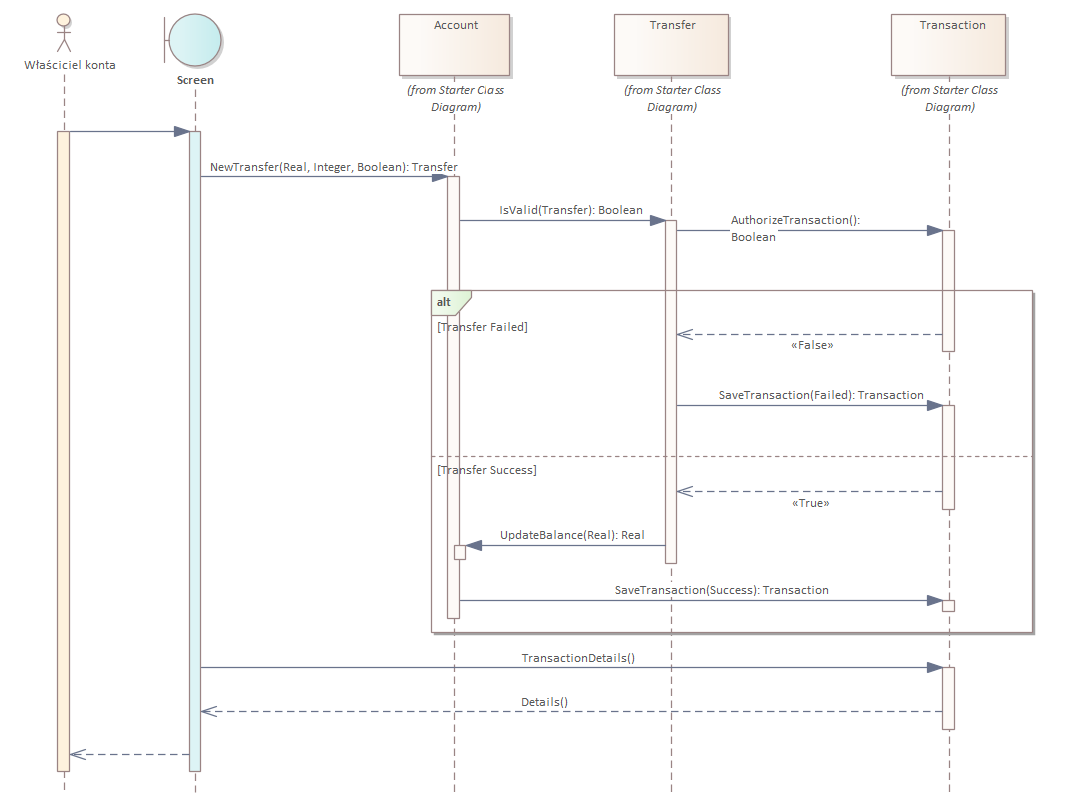
\includegraphics[width=0.7\textwidth]{images/Przelew.png}
	\caption{Diagram sekwencji Przelew}
	\label{fig:Seq2}
\end{figure}